
How do \emph{ad hoc} conventions formed through interaction with a single partner become \emph{global} conventions shared throughout a community?
In this section, we provide an explicit computational account of the cognitive mechanisms driving this shift.
The key predictions distinguishing our model concern the pattern of generalization across partners.
First, we show that our model accounts for the \emph{partner-specificity} of ad hoc conventions as a consequence of hierarchical structure. 
Under our model, speakers revert back to a longer description with a novel partner because evidence from a single listener is relatively uninformative about the community-level prior.

This hierarchical structure, however, leads to a further prediction: after interacting with enough partners in a tight-knit community, speakers should become increasingly confident that labels are not simply idiosyncratic features of a particular partner's lexicon but are shared across the entire community.
In other words, the partner-specific expectations agents form within an interaction to solve a novel communication problem should gradually generalize to community-wide expectations as they gain additional evidence of the latent population-level distribution from which different partners are sampled.
These expectations should manifest in an increasing willingness to use short labels with novel partners, leading to the emergent consequence of lending additional evidence for that structure. 
We test this novel prediction in a networked communication game and compare our model to two non-hierarchical variants: a `complete-pooling' model that collapses across partners and a `no-pooling' model that treats partners as entirely separate.

\subsection{Model predictions}

\begin{figure*}
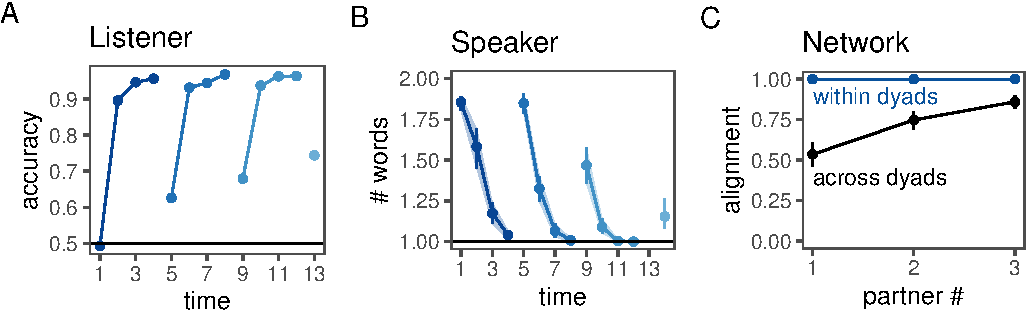
\includegraphics[scale=1]{./figures/sec3-model_results.pdf}
\caption{Simulation results for (A) listener accuracy, (B) speaker reduction, and (C) network convergence across three partners.}
\label{fig:model_results}
\end{figure*}

We investigate the generalization behavior of our model under three increasingly complex scenarios. 
In all of these scenarios, speaker and listener agents play a reference game with a set of two objects $\{o_1, o_2\}$.
On each trial, one of these objects is designated for the speaker as the *target*. 
They must select from a set of utterances $\{u_0, \dots, u_j\}$ to convey the identity of the target to the listener.
Upon hearing this utterance, the listener selects which of the objects they believe to be the target and then receives feedback about the true target.
The resulting data $D_k$ from an interaction with partner $k$ thus consists of utterance-object pairs $\{(u, o)_t\}$ for each trial $t$, as well as information about the context of objects.

Given this reference game setting, we can explicitly specify the likelihood and prior terms. 
We consider a likelihood given by the Rational Speech Act (RSA) framework, which formalizes the Gricean assumption of cooperativity \cite{GoodmanFrank16_RSATiCS}.
A pragmatic speaker $S_1$ attempts to trade off informativity against the cost of producing an utterance, while a pragmatic listener $L_1$ inverts their model of the speaker to infer the intended target.
The chain of recursive social reasoning grounds out in a \emph{literal listener} $L_0$, who identifies an intended meaning using their lexical knowledge $\mathcal{L}_{\phi_k}$. 
This model can be formally specified as follows:
$$
\begin{array}{rcl}
L_0(o | u, \phi_k) &\propto  & \exp\{\mathcal{L}_{\phi_k}(u,o)\} \\
S_1(u | o, \phi_k) &\propto &  \exp\{w_I \cdot \log L_0(o | u, \phi_k) - w_C \cdot \textrm{cost}(u)\}   \\
L_1(o | u, \phi_k) &\propto  & S_1(u | o, \phi_k) P(o) 
\end{array}
$$
where $w_I$ and $w_C$ are free parameters controlling the relative weights on the informativity and parsimony, respectively\footnote{Throughout our simulations, we set $w_I = 11,~w_C = 7$. A grid search over parameter space revealed different regimes of behavior, but we leave broader exploration of this space to future work.}
We define $P(D_k | \phi_k)$ as the probability of the data under a pragmatic listener $L_1$.
We also use this RSA model to simulate the behavior of uncertain speakers $S$ and listeners $L$. 
Utterances and object selections are sampled from the posterior predictive, marginalizing over lexical uncertainty.

Finally, we must specify the form of the lexical prior and a method to perform inference in this model.
We assume $\Theta$ is a matrix with an entry for each utterance-object pair $(u_i, o_j)$, and use independent Gaussian distributions for each $\Theta_{ij} \in \Theta$ as a hyper-prior.
We then centered our partner-specific prior $\phi_{ij} \in \phi$ at the shared value for a particular partner:
$$\begin{array}{rcl}
P(\Theta_{ij}) & \sim & \mathcal{N}(0, 1)\\
P(\phi_{ij} | \Theta_{ij}) & \sim & \mathcal{N}(\Theta_{ij}, 1)
\end{array}$$
These priors represent assumptions about how far partner-specific learning can drift from the community-wide value.

For all simulations, we used the implementation of variational inference in WebPPL \cite{GoodmanStuhlmuller14_DIPPL}
Variational methods transform probabilistic inference problems into optimization problems by approximating the true posterior with a parameterized family.
Specifically, we make a \emph{mean-field} approximation and assume that the full posterior can be factored into independent Gaussians for each random variable. 
We then optimize the parameters of these posterior Gaussians by minimizing the evidence lower bound (ELBO) objective.
We run 50,000 steps of gradient descent on the first observation to obtain a posterior, compute the agent's marginal prediction for the next observation by taking the expectation over 50,000 samples from the posterior predictive, then resume gradient descent on the resulting outcome.

\paragraph{Simulation 1: Listener accuracy across partners}

The key predictions of our model concern the pattern of generalization across partners.
In our first simulation, we consider the partner-specificity of a *listener*'s expectations about which object is being referred to.
To observe the model's behavior in the simplest case, we assume the speaker has a vocabulary of two single-word utterances $\{u_1, u_2\}$ with equal cost and use the same utterance and target object ($\{o_1, u_1\}$) on every trial.
We introduce a new partner every 4 trials.

The probability assigned to the target on each trial is shown in Fig. \ref{fig:model_results}A.
The listener model begins at chance due to its uninformative prior, but after observing several trials of evidence from the same partner, it rapidly infers the meaning of $u_1$ and learns to choose the true target with high accuracy.
When a second partner is introduced, however, it reverts nearly to its original state.
This reversion is due to ambiguity about whether the behavior of the first partner was idiosyncratic or attributable to community-level conventions.
In the absence of data from other partners, this data is more parsimoniously explained with a partner-specific model.
After observing multiple partners behave similarly, however, we find that this knowledge has gradually been incorporated into community-level expectations. 
This is evident in much stronger initial expectations by the fourth partner ($\sim$ 75\% accuracy vs. 50\% with the first partner.)

\paragraph{Simulation 2: Speaker utterance length across partners}

Next, we examined our model's predictions about how a *speaker*'s referring expressions will change with successive listeners.
While it has been frequently observed that messages reduce in length across repetitions with a single partner and sharply revert back to longer utterances when a new partner is introduced \cite{wilkes-gibbs_coordinating_1992}, the key prediction distinguishing our model concerns behavior across subsequent partner boundaries.
Complete-pooling accounts predict no change in number of words when a new partner is introduced.
No-pooling accounts predict that roughly the same initial description length will re-occur with every subsequent interlocutor. 
Here we show that a partial pooling account predicts a more complex pattern of generalization.

We allowed a set of four primitive utterances, $\{u_1, u_2, u_3, u_4\}$, to be combined into conjunctions, e.g. $\{u_1+u_2, u_3+u_4\}$, which are assumed to have a higher utterance cost.
The meanings of these conjunctions were determined compositionally from the values of the primitive utterances\footnote{We used a standard product T-norm for conjunction. Because our values come from a Gaussian prior and the T-norm is defined over $[0,1]$, we used logistic and logit function to map values to the unit interval and back.}
Speakers do not typically begin at chance over their *entire* vocabulary, so we used a weakly biased prior for $\Theta$: two of the primitive utterances initially applied more strongly to $o_1$ and the other two more strongly to $o_2$.
This weak bias leads to a preference for conjunctions at the outset and thus allows us examine reduction.

We paired the speaker model with a fixed listener who always selected the target, and ran 48 independent simulations.
First, we found that descriptions become more efficient over interaction with a single partner: the model becomes more confident that shorter utterances will be meaningful, so the marginal informativity provided by the conjunction is not worth the additional cost (see Sec.~\ref{sec:dyadic}).
Critically, we find that the speaker model reverts back to a longer description at the first partner swap: evidence from one partner is relatively uninformative about the community.
After interacting with several partners, however, it becomes more likely that one of the short labels is shared across the entire community, and the model is correspondingly more likely to begin a new interaction with it (Fig. \ref{fig:model_results}B).

\paragraph{Simulation 3: Network convergence}

The first two simulations presented a single adaptive agent with a fixed partner to understand its gradient of generalization. 
In our final simulation, we test the consequences of the proposed hierarchical inference scheme for a network of interacting agents.
From each individual agent's perspective, this simulation is identical to the earlier ones (i.e. a sequence of 3 different partners).
Because all agents are simultaneously making inferences about the others, however, the network as a whole faces a coordination problem.
For example, in the first block, agents 1 and 2 may coordinate on using $u_1$ to refer to $o_1$ while agent 3 and 4 coordinate on using $u_2$. 
Once they swap partners, they must negotiate this potential mismatch in usage. 
How does the network as a whole manage to coordinate?

We used a round-robin scheme to schedule four agents into three blocks of interaction, with each agent taking turns in the speaker and listener roles, and simulated 48 networks.
We measured alignment by computing whether different agents produced the same one-word utterances. 
We compared the alignment between currently interacting agents (i.e. *within* a dyad) to those who were not interacting (i.e. *across* dyads).
Alignment across dyads was initially at chance, reflecting the arbitrariness of whether speakers reduce to $u_1$ or $u_2$. 
In the absence of hierarchical generalization, we would expect subsequent blocks to remain at chance, as pacts would need to be re-negotiated from scratch.
Instead, we find that alignment across dyads gradually increases, suggesting that partial pooling leads to emergent consensus (Fig. \ref{fig:model_results}C).

\subsection{Behavioral methods}

\begin{figure*}
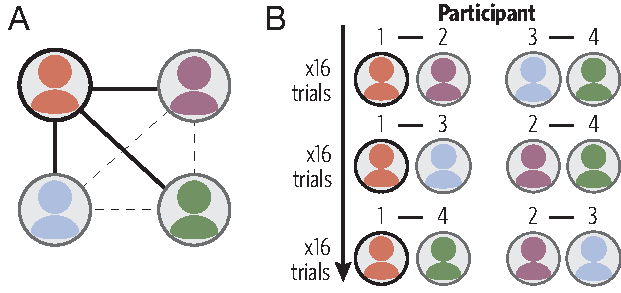
\includegraphics[scale=1]{./figures/sec3-design.pdf}
\caption{In our experiment, (A) participants were placed in fully-connected networks of 4, (B) paired in a round-robin schedule  with each neighbor, and (C) played a series of repeated reference games using tangram stimuli.}
\label{fig:task1_display}
\end{figure*}

To evaluate the qualitative predictions observed in our simulations, we designed a natural-language communication experiment following roughly the same network design.
Instead of anonymizing partners, as in many previous empirical studies of convention formation, we divided the experiment into blocks of extended dyadic interactions with stable, identifiable partners \cite<see>[for similar designs]{fay_interactive_2010; garrod_conversation_1994}.
Each block was a full repeated reference game, where participants had to coordinate on an *ad hoc* convention, or *pact*, for how to refer to novel objects with their partner \cite{BrennanClark96_ConceptualPactsConversation}.
Our model predicts that these pacts will reset at partner boundaries, but that agents should be increasingly willing to transfer expectations from one partner to another.

\paragraph{Participants}

We recruited 92 participants from Amazon Mechanical Turk to play a series of interactive, natural-language reference games.

\paragraph{Stimuli and procedure}

Each participant was randomly assigned to one of `r numNetworks` fully-connected networks with three other participants as their 'neighbors' (Fig. \ref{fig:task1_display}A). 
Each network was then randomly assigned one of three distinct "contexts" containing abstract tangram stimuli taken from \citeA{clark_referring_1986}.
The experiment was structured into a series of three repeated reference games with different partners, using these same four stimuli as referents.
Partner pairings were determined by a round-robin schedule (Fig. \ref{fig:task1_display}B).
The trial sequence for each reference game was composed of four repetition blocks, where each target appeared once per block.
After completing sixteen trials with one partner, participants were introduced to their next partner and asked to play the game again. 
This process repeated until each participant had partnered with all three neighbors.
Because some pairs within the network took longer than others, we sent participants to a temporary waiting room if their next partner was not ready. 

Each trial proceeded as follows.
First, one of the four tangrams in the context was highlighted as the \emph{target object} for the "speaker." 
They were instructed to use a chatbox to communicate the identity of this object to their partner, the "listener" (see Fig. \ref{fig:task1_display}C).
The listener could reply freely through the chatbox but was asked to ultimately make a selection from the array. 
Finally, both participants in a pair were given full feedback on each trial about their partner's choice and received bonus payment for each correct response. 
The order of the stimuli on the screen was randomized on every trial to prevent the use of spatial cues (e.g. 'the one on the left').
The display also contained an avatar representing their current partner to emphasize that they were speaking to the same partner for an extended period.

\subsection{Results}

\begin{figure*}
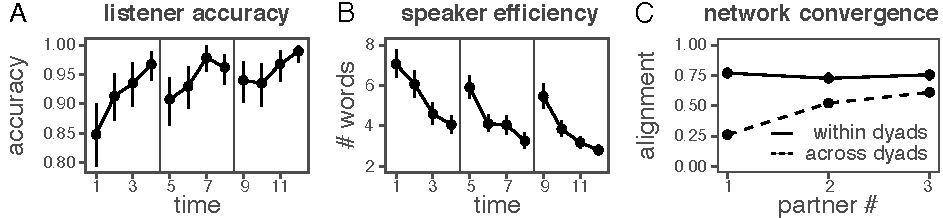
\includegraphics[scale=1]{./figures/sec3-empirical-results.pdf}
\caption{Results from networked communication experiment. (A) Increase in accuracy across partners, (B) reduction in number of words across partners, (C) network convergence.}
\label{fig:results}
\end{figure*}

We evaluated participants' generalization behavior on the same three metrics we used in our simulations: accuracy, utterance length, and network convergence.

\paragraph{Listener accuracy}

We first examined changes in the proportion of correct listener selections.
In particular, our partial pooling model predicts (1) gains in accuracy within each partner and (2) drops in accuracy at partner boundaries, but (3) overall improvement in initial interactions with successive partners.
To test the first prediction, we constructed a logistic mixed-effects regression predicting trial-level listener responses. 
We included a fixed effect of repetition block within partner (1, 2, 3, 4), along with random intercepts and slopes for each participant and each tangram. 
We found that accuracy improved over successive repetitions with every partner, $b=0.69,z=3.87, p<0.001$.

To test changes at partner boundaries, we constructed another regression model.
We coded the repetition blocks immediately before and after each partner swap, and included this as a categorical fixed effect.
Because partner roles were randomized for each game, the same participant often did not serve as listener in both blocks, so in addition to tangram-level intercepts, we included random slopes and intercepts at the *network* level (instead of the participant level).
We found that across the two partner swaps, accuracy dropped significantly, $b = -1.56, z = -2, p < 0.05$, reflecting partner-specificity of meaning.
Finally, to test whether performance in the initial repetition block improves with subsequent partners, we examined the simple effect of partner number, restricting analysis to the first repetition block.
As predicted, we found a significant improvement in performance, $b = 0.57, z = 2.72, p < 0.01$, suggesting that listeners are bringing increasingly well-calibrated expectations into interactions with novel neighbors (see Fig. \ref{fig:results}A).


\paragraph{Speaker utterance length}

Next, as a measure of coding efficiency, we calculated the raw number of words produced by a speaker on each trial.
We then tested analogs of the same three predictions we tested in the previous section using the same mixed-effects models, but using (log) utterance length as a continuous DV instead of accuracy (see Fig. \ref{fig:results}B).
We found that speakers reduced utterance length with every partner, $b = -0.19, t(34) = -9.88, p < 0.001$, increased length across partner-boundaries, $b = 0.43, t(22) = 4.4, p < 0.001$, and decreased the length of their initial descriptions as they interacted with more partners on their network, $b = -0.2, t(516.5) = -6.07, p < 0.001$ (see Fig. \ref{fig:results}B).

\paragraph{Network convergence }

In this section, we examine the actual *content* of pacts and test whether these coarse signatures of generalization actually lead to increased alignment across the network, as predicted. 
Specifically, we extend the 'exact matching' measure of alignment used in Simulation 3 to natural language production by examining whether the *intersection* of words produced by different speakers was non-empty\footnote{We excluded a list of common stop words (e.g. 'the', 'both') to focus on the core conceptual content of pacts; using the size of the intersection instead of the binary variable yielded similar results.}
As in our simulation, the main comparison of interest was between currently interacting participants and participants who are not interacting: we predicted that within-pair alignment should stay consistently high while (tacit) alignment between non-interacting pairs will increase. 
We thus constructed a mixed-effects logistic regression including fixed effects of pair type (within vs. across), partner number, and their interaction.
We included random intercepts at the tangram level and maximal random effects at the network level (i.e. intercept, both main effects, and the interaction).
As predicted, we found a significant interaction ($b = -0.85, z = -5.69, p < 0.001$; see Fig. \ref{fig:results}C).
Although different pairs in a network may initially use different labels, these labels begin to align over subsequent interactions. 

\subsection{Discussion}

How do community-level conventions emerge from local interactions? 
Our partial pooling model claims that conventions represent the shared structure that agents "abstract away" from partner-specific learning.
In this section, we evaluated the extent to which our partial pooling model captured human generalization behavior in a natural-language communication experiment on small networks.
Unlike complete-pooling accounts, our model allows for partner-specific common ground to override community-wide expectations given sufficient experience with a partner, or in the absence of strong conventions.
Unlike no-pooling accounts, it allows networks to converge on more efficient and accurate expectations about novel partners.

Hierarchical Bayesian models have several other properties of theoretical interest for convention formation.
First, they offer a "blessing of abstraction" \cite{GoodmanUllmanTenenbaum11_TheoryOfCausality}, where community-level conventions may be learned even with relatively sparse input from each partner, as long as there is not substantial variance in the population. 
Second, they are more robust to partner-specific deviations from conventions (e.g. interactions with children or non-native speakers) than complete-pooling models relying on a fixed set of memory slots or a single mental 'inventory.' 
This robustness is due to their ability to 'explain away' outliers without community-level expectations being affected. 
Finally, the deep connection between hierarchical Bayesian models and accounts of *meta-learning*, or learning to learn \cite{grant_recasting_2018}, provides a useful set of tools to analyze conventions as the result of agents solving a meta-learning problem, adapting to each partner along the way.
